






\subsection*{Machine Learning Integration}

It is common for companies to develop their own in-house game engines and subsequently build their applications on these platforms. However, the integration of pre-installed machine learning components is less prevalent.

Typically, integrating machine learning into games involves installing complex extensions over pre-existing game engines.

\subsubsection*{inWorld AI}
InWorld AI is an example of such a service. It provides installable extensions for popular game engines and offers an interface for communicating with pre-trained OpenAI agents. This solution is excellent for facilitating human-to-AI communication, making it ideal for dialogues and NPC integration.

\begin{figure}[h]
\centering
\begin{minipage}[t]{0.48\textwidth}
\centering
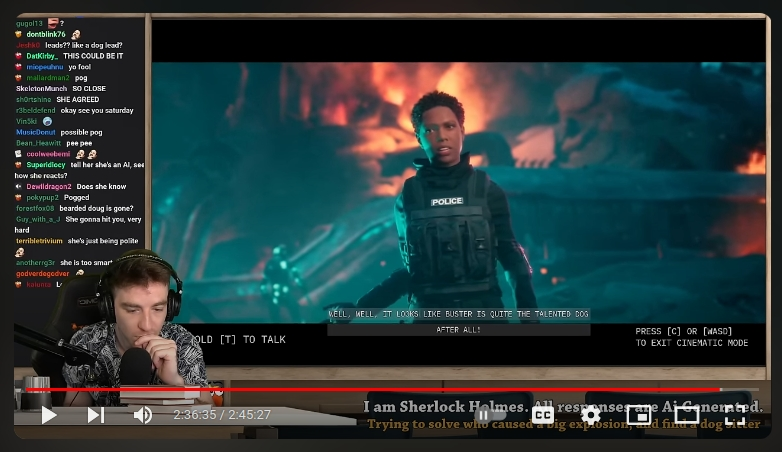
\includegraphics[width=\textwidth, height=5cm]{dougdoug}
\caption{inWorld Ai Demo}
\end{minipage}%
\hfill
\begin{minipage}[t]{0.48\textwidth}
\centering
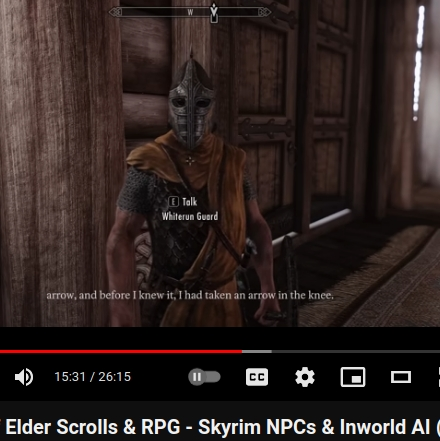
\includegraphics[width=\textwidth, height=5cm]{arrow.jpeg}
\caption{inWorld Ai Demo}
\end{minipage}
\end{figure}

\subsubsection*{Interactive Simulacra of Human Behavior}

Another notable example is this research paper that successfully trained multiple ML agents to interact within a pre-created world. These agents are capable of remembering conversations and interactions and can even organize activities amongst themselves.

\begin{figure}[h]
    \centering
    \begin{minipage}[t]{0.48\textwidth}
        \centering
        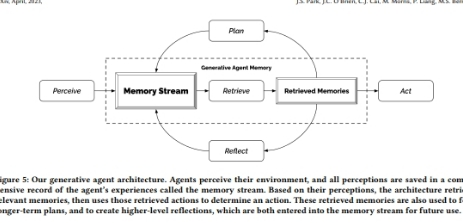
\includegraphics[height= 0.5 \textwidth]{DataStructure.jpeg}
        \caption{Data structure used for memory management}
        % \label{fig:image1}
    \end{minipage}%
    \hfill
    \begin{minipage}[t]{0.48\textwidth}
        \centering
        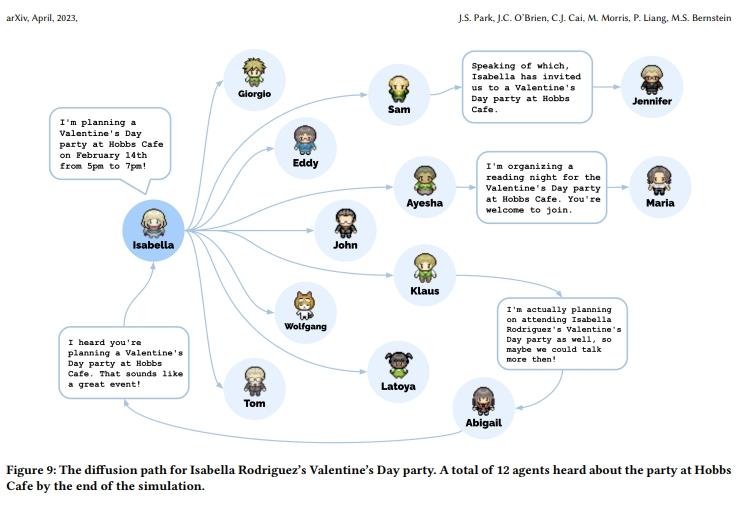
\includegraphics[height= 0.5 \textwidth]{birthdayParty.jpeg}
        \caption{One Agent organised a birthday party}
        % \label{fig:image2}
    \end{minipage}
\end{figure}


By integrating these advanced machine learning solutions, game developers can significantly enhance the immersion and interactivity of their NPCs, creating more engaging and dynamic gameplay experiences.
